\documentclass[a4paper,colorlinks=true,linkcolor=blue,urlcolor=blue,citecolor=green,bookmarks=true]{article}

% 基础宏包
\usepackage{ctex}              % 中文支持
\usepackage{graphicx}          % 图片支持
\usepackage{amsmath}           % 数学公式
\usepackage{amssymb}          % 数学符号
\usepackage{geometry}          % 页面设置
\usepackage{fancyhdr}          % 页眉页脚
\usepackage{lastpage}          % 获取总页数
\usepackage{zhnumber}          % 中文数字
\usepackage{float}             % 浮动体设置
\usepackage{subcaption}        % 支持子图

% 页面设置
\geometry{a4paper,top=2.5cm,bottom=2.5cm,left=2.5cm,right=2.5cm}

% 浮动体设置
\renewcommand{\textfraction}{0.05}
\renewcommand{\topfraction}{0.95}
\renewcommand{\bottomfraction}{0.95}
\renewcommand{\floatpagefraction}{0.35}
\setcounter{topnumber}{5}
\setcounter{bottomnumber}{5}
\setcounter{totalnumber}{10}

% 引入样式文件
% 基础包引用
\usepackage{amsmath}
\usepackage{graphicx}
\usepackage{float}
\usepackage{setspace}
\usepackage{xargs}
\usepackage{nameref}
\usepackage{appendix}
\usepackage{cite}
\usepackage{hyperref}
\usepackage{fancyref}
\usepackage{scrextend}

% 颜色定义
\usepackage[dvipsnames]{xcolor}
\definecolor{cleanOrange}{HTML}{D14D00}
\definecolor{cleanYellow}{HTML}{FFFF99}
\definecolor{cleanBlue}{HTML}{3d0099}

% 通用命令
\newcommand\tab[1][1cm]{\hspace*{#1}}
\hypersetup{colorlinks=true, linkcolor=black}
\interfootnotelinepenalty=10000

% 注释和标记
\usepackage[colorinlistoftodos,prependcaption,textsize=footnotesize]{todonotes}
\newcommandx{\commred}[2][1=]{\textcolor{Red}{\todo[linecolor=red,backgroundcolor=red!25,bordercolor=red,#1]{#2}}}
\newcommandx{\commblue}[2][1=]{\textcolor{Blue}{\todo[linecolor=blue,backgroundcolor=blue!25,bordercolor=blue,#1]{#2}}}
\newcommandx{\commgreen}[2][1=]{\textcolor{OliveGreen}{\todo[linecolor=OliveGreen,backgroundcolor=OliveGreen!25,bordercolor=OliveGreen,#1]{#2}}}
\newcommandx{\commpurp}[2][1=]{\textcolor{Plum}{\todo[linecolor=Plum,backgroundcolor=Plum!25,bordercolor=Plum,#1]{#2}}}

% 代码和注释
\def\code#1{{\tt #1}}
\def\note#1{\noindent{\bf [Note: #1]}}

% 附录格式
\makeatletter
\def\@seccntformat#1{\@ifundefined{#1@cntformat}%
   {\csname the#1\endcsname\quad}%
   {\csname #1@cntformat\endcsname}%
}
\let\oldappendix\appendix
\renewcommand\appendix{%
    \oldappendix
    \newcommand{\section@cntformat}{\appendixname~\thesection\quad}
}
\makeatother 
% 页面布局设置
\usepackage{geometry}
\geometry{a4paper,left=2.3cm,right=2.3cm,top=2.7cm,bottom=2.7cm}

% 页眉页脚
\usepackage{fancyhdr}
\usepackage{lastpage}
\pagestyle{fancy}
\renewcommand{\headrulewidth}{0.1pt}
\renewcommand{\footrulewidth}{0pt}

% 章节格式
\usepackage{sectsty}
\sectionfont{\LARGE}
\subsectionfont{\Large}
\subsubsectionfont{\large}

% 表格设置
\usepackage{tabularx}
\usepackage{booktabs}
\usepackage{multirow}

% 图表设置
\usepackage{caption}
\usepackage{subfigure}
\setlength{\textfloatsep}{10mm}

% 标题线设置
\providecommand{\HRule}{\rule{\linewidth}{0.5mm}}
\providecommand{\HRulegrossa}{\rule{\linewidth}{1.2mm}} 
% 字体和编码设置
\usepackage{ctex}
\usepackage[utf8]{inputenc}
\usepackage[british,UKenglish]{babel}

% 字体命令
\newcommand{\cleancode}[1]{\begin{addmargin}[3em]{3em}\texttt{\textcolor{cleanOrange}{#1}}\end{addmargin}}
\newcommand{\cleanstyle}[1]{\text{\textcolor{cleanOrange}{\texttt{#1}}}} 
% 代码样式设置
\usepackage[T1]{fontenc}
\usepackage[scaled=0.82]{beramono}
\usepackage{microtype}
\usepackage[procnames]{listings}

% 代码颜色定义
\definecolor{dkgreen}{rgb}{0,0.6,0}
\definecolor{gray}{rgb}{0.5,0.5,0.5}
\definecolor{mauve}{rgb}{0.58,0,0.82}

% 基础代码样式
\lstset{
  frame=tb,
  aboveskip=3mm,
  belowskip=3mm,
  showstringspaces=false,
  columns=fixed,
  basicstyle={\small\ttfamily},
  numbers=left,
  numberstyle=\tiny\color{gray},
  keywordstyle=\color{blue},
  commentstyle=\color{dkgreen},
  stringstyle=\color{mauve},
  frame=single,
  breaklines=true,
  breakatwhitespace=true,
  tabsize=2
}

% Scala语言定义
\lstdefinelanguage{scala}{
  morekeywords={abstract,case,catch,class,def,
    do,else,extends,false,final,finally,
    for,if,implicit,import,match,mixin,
    new,null,object,override,package,
    private,protected,requires,return,sealed,
    super,this,throw,trait,true,try,
    type,val,var,while,with,yield},
  sensitive=true,
  morecomment=[l]{//},
  morecomment=[n]{/*}{*/},
  morestring=[b]",
  morestring=[b]',
  morestring=[b]"""
}

% 语言环境定义
\lstnewenvironment{scala}[1][]
{\lstset{language=scala,#1}}
{}
\lstnewenvironment{cpp}[1][]
{\lstset{language=C++,#1}}
{}
\lstnewenvironment{bash}[1][]
{\lstset{language=bash,#1}}
{}
\lstnewenvironment{verilog}[1][]
{\lstset{language=verilog,#1}}
{} 

% 图片路径
\graphicspath{{fig/}}

% 使用natbib和plainurl风格
\usepackage[numbers,sort&compress,square,comma]{natbib}
\bibliographystyle{unsrtnat}

% 参考文献处理增强
\usepackage{hyperref}
\usepackage{url}
\usepackage{xurl}
\renewcommand{\UrlFont}{\ttfamily\color{blue}\small}

% 确保文献内含中文字符时正确编译
\usepackage{etoolbox}
\patchcmd{\thebibliography}{\sloppy}{\sloppy\raggedright}{}{}

% 自定义参考文献样式
\makeatletter
\renewcommand\@biblabel[1]{{\bf [#1]}}
\def\@cite#1#2{[{#1\if@tempswa , #2\fi}]}
\renewcommand{\bibfont}{\small}
\setlength{\bibsep}{1.2ex}
\makeatother

% 美化URL显示
\usepackage{xurl}
\renewcommand{\UrlFont}{\ttfamily\color{blue}\small}

% 伪代码设置
\usepackage{algorithm}  
\usepackage{algorithmicx}  
\usepackage{algpseudocode}  
\floatname{algorithm}{Algorithm}  
\renewcommand{\algorithmicrequire}{\textbf{Input:}}  
\renewcommand{\algorithmicensure}{\textbf{Output:}} 
\usepackage{lipsum}  

% 定义中英文摘要环境
\makeatletter
% 中文摘要环境
\newenvironment{cnabstract}{
    \par\small
    \noindent\mbox{}\par\vspace{-\baselineskip}
    \par\songti\parindent 2em
    }
    {\par\vspace{1em}}

% 英文摘要环境
\newenvironment{enabstract}{
    \par\small
    \noindent\mbox{}\par\vspace{-\baselineskip}
    \par\parindent 2em
    }
    {\par\vspace{1em}}
\makeatother

\makeatletter
\providecommand{\breakablealgorithm}{%
  \begin{center}
     \refstepcounter{algorithm}%
     \hrule height.8pt depth0pt \kern2pt%
     \renewcommand{\caption}[2][\relax]{%
      {\raggedright\textbf{\ALG@name~\thealgorithm} ##2\par}%
      \ifx\relax##1\relax
         \addcontentsline{loa}{algorithm}{\protect\numberline{\thealgorithm}##2}%
      \else
         \addcontentsline{loa}{algorithm}{\protect\numberline{\thealgorithm}##1}%
      \fi
      \kern2pt\hrule\kern2pt
     }
  \end{center}
}
\makeatother

%-------------------------页眉页脚--------------
\pagestyle{fancy}
\lhead{\kaishu \leftmark}
\rhead{\kaishu 并行程序设计实验报告}
\lfoot{}
\cfoot{\thepage}
\rfoot{}

%--------------------文档内容--------------------

\begin{document}
\renewcommand{\contentsname}{目录}
\renewcommand{\appendixname}{附录}
\renewcommand{\appendixpagename}{附录}
\renewcommand{\refname}{参考文献} 
\renewcommand{\figurename}{图}
\renewcommand{\tablename}{表}
\renewcommand{\abstractname}{摘要}
\renewcommand{\today}{\number\year 年 \number\month 月 \number\day 日}

\renewcommand {\thefigure}{\thesection{}.\arabic{figure}}%图片按章标号
\renewcommand{\figurename}{图}
\renewcommand{\contentsname}{目录}  
\cfoot{\thepage\ of \pageref{LastPage}}%当前页 of 总页数

% 封面
\begin{titlepage}
    \begin{center}
    
\includegraphics[width=0.6\textwidth]{NKU.png}\\[1cm]
    \vspace{20mm}
		\textbf{\huge\textbf{\kaishu{计算机学院}}}\\[0.5cm]
		\textbf{\huge{\kaishu{并行程序设计报告}}}\\[2.3cm]
		\textbf{\Huge\textbf{\kaishu{NTT SIMD优化实验报告}}}

		\vspace{\fill}
    
    \centering
    \textsc{\LARGE \kaishu{姓名\ :\ 廖望}}\\[0.5cm]
    \textsc{\LARGE \kaishu{学号\ :\ 2210556}}\\[0.5cm]
    \textsc{\LARGE \kaishu{专业\ :\ 计算机科学与技术}}\\[0.5cm]
    
    \vfill
    {\Large \today}
    \end{center}
\end{titlepage}

% 中文摘要
\clearpage
\phantomsection
\begin{center}{\zihao{4}\songti\bfseries{摘\quad 要}}\end{center}\par\vspace{0.5em}
\addcontentsline{toc}{section}{摘要}
\begin{cnabstract}
本报告探讨了数论变换(NTT)的SIMD优化实现,重点研究不同优化策略在x86-64(AVX2)和ARM(NEON)平台上的性能表现。我们实现了朴素NTT、DIF结构优化、SIMD向量化以及DIF+SIMD联合优化四种方案,并在不同模数(469762049、1337006139375617和7696582450348003)下进行了性能对比。实验结果表明:1)在AVX2平台(256位宽向量寄存器)上,DIF+AVX2联合优化在标准模数下提供了约35\%的加速;2)在NEON平台(128位宽向量寄存器)上,DIF结构优化表现最佳,提供了约4倍加速,而DIF+NEON联合优化反而性能下降;3)对于超大模数,我们探索了基于中国剩余定理的拼接技术,成功实现了SIMD优化。本研究揭示了硬件特性与算法结构的匹配关系对优化效果的关键影响,为多项式乘法在密码学等领域的高效实现提供了重要参考。附录中提供了NEON平台的实验结果截图。代码仓库可访问:\href{https://github.com/aokimi0/parallel-programming}{GitHub}。

\vspace{1em}
\noindent\textbf{关键词:}数论变换;SIMD优化;向量化计算;多项式乘法;蝴蝶变换
\end{cnabstract}

% 英文摘要
\phantomsection
\begin{center}{\zihao{4}\bfseries{Abstract}}\end{center}\par\vspace{0.5em}
\addcontentsline{toc}{section}{Abstract}
\begin{enabstract}
This report investigates SIMD optimization strategies for Number Theoretic Transform (NTT), focusing on performance across x86-64 (AVX2) and ARM (NEON) platforms. We implemented four versions: naive NTT, DIF-structured optimization, SIMD vectorization, and combined DIF+SIMD optimization, testing them with different moduli (469762049, 1337006139375617, and 7696582450348003). Results show that: 1) On the AVX2 platform (256-bit vector registers), DIF+AVX2 joint optimization achieved approximately 35\% speedup for standard moduli; 2) On the NEON platform (128-bit vector registers), DIF structural optimization provided the best performance with a 4-fold acceleration, while surprisingly, the DIF+NEON joint optimization performed worse than DIF alone; 3) For large moduli, we explored a Chinese Remainder Theorem-based technique that successfully implemented SIMD optimization. This study reveals the critical impact of matching hardware characteristics with algorithm structure, providing important references for efficient polynomial multiplication implementation in cryptography and other fields. Experimental result screenshots for the NEON platform are provided in the appendix. Full code is available at: \href{https://github.com/aokimi0/parallel-programming}{GitHub}.

\vspace{1em}
\noindent\textbf{Keywords:} Number Theoretic Transform; SIMD Optimization; Vectorized Computing; Polynomial Multiplication; Butterfly Operation
\end{enabstract}

% 目录
\clearpage
\tableofcontents
\clearpage

\section{问题描述}

\subsection{研究背景}
多项式乘法是信号处理、计算机图形学、密码学等领域的基础运算,尤其在同态加密等安全领域中具有重要作用。同态加密可以在密文上进行运算,对运算后的密文进行解密的结果等于明文直接运算的结果,这在隐私保护和安全计算中至关重要。传统的多项式乘法算法复杂度为$O(n^2)$,难以满足大规模数据处理需求。快速数论变换(NTT)作为FFT在有限域上的变体,能够将复杂度降低到$O(n\log n)$,并避免了浮点误差问题。

\subsection{本实验子问题}
本实验聚焦于多项式乘法的NTT优化,特别是利用SIMD指令集对NTT算法进行向量化加速。主要目标包括:
\begin{itemize}
  \item 实现NTT的高效并行化,提升多项式乘法性能
  \item 探索向量化取模、蝴蝶变换等关键步骤的SIMD优化方法
  \item 通过性能剖析工具分析SIMD优化的效果
  \item 对比串行与SIMD优化下的性能差异
\end{itemize}

\section{SIMD算法设计与实现}

\subsection{NTT算法原理}
NTT(Number Theoretic Transform)是将FFT的复数单位根替换为有限域上的单位根,所有运算均在模$p$的有限域$Z_p$上进行。对于质数$p$,我们定义$Z_p=\{0,1,2,...,p-1\}$,其中元素的加减乘运算均在模$p$下进行\cite{harvey2014}。

NTT的关键是选择适当的模数$p$和原根$g$,使得$n|(p-1)$,其中$n$是变换长度(通常为2的幂次)。在本实验中,我们使用的模数均满足$p = a \times 4^k + 1$的形式,且原根均为3\cite{longa2016}。

\subsubsection{超大模数处理探索}

超大模数如1337006139375617会超出32位整数表示范围,直接用SIMD指令处理会面临困难。而对于7696582450348003这样的特殊模数,我们探索了一种基于中国剩余定理(CRT)的处理方法:

\begin{enumerate}
  \item 将这类模数分解为较小的NTT友好模数(如7340033和104857601)
  \item 分别在这些小模数下执行SIMD优化的NTT
  \item 使用中国剩余定理合并结果
\end{enumerate}

例如,7696582450348003可表示为两个小模数的乘积近似值:
$7696582450348003 \approx 7340033 \times 104857601$

对于多项式$A$和$B$,我们可以:
\begin{itemize}
  \item 计算$A \times B \mod 7340033$,得到结果$R_1$
  \item 计算$A \times B \mod 104857601$,得到结果$R_2$
  \item 使用CRT重建最终结果$R$,满足$R \equiv R_1 \pmod{7340033}$且$R \equiv R_2 \pmod{104857601}$
\end{itemize}

这种方法充分利用了SIMD指令在小模数下的高效性,解决了超大模数计算的问题。

\subsection{SIMD优化思路}
NTT的主要计算瓶颈在于大量的加法、减法和模乘操作。SIMD优化的关键在于:
\begin{itemize}
  \item \textbf{向量化加减法}:利用SIMD指令一次处理多个数据元素,加速蝴蝶变换中的加减操作\cite{intel-avx2};
  \item \textbf{向量化取模}:由于SIMD指令不直接支持取模,需要采用分支、近似或Montgomery规约等方法实现高效模乘;
  \item \textbf{向量化蝴蝶变换}:将NTT迭代实现中的内层循环用SIMD指令替换,提升并行度\cite{zhang2022}。
  \item \textbf{DIF(Decimation-In-Frequency)优化}:DIF是一种按频率抽取的NTT实现方式,与DIT(按时间抽取)相比,DIF在数据访问和内存布局上更适合SIMD向量化\cite{wu2023}。DIF优化能够减少位翻转操作,提升数据局部性,使得SIMD指令能够更高效地批量处理数据,进一步提升整体性能。
\end{itemize}

\subsubsection{向量化取模}
SIMD指令集通常不直接支持取模操作,需要特殊处理:
\begin{itemize}
  \item \textbf{Montgomery规约}:将模乘转化为一系列加减乘和位运算,适合SIMD实现
  \item \textbf{浮点近似取模}:通过浮点除法近似取模运算,在某些场景下有效
  \item \textbf{分支处理}:针对超出模数的情况进行条件分支处理
\end{itemize}

本实验主要采用Montgomery规约方法,它能将模乘操作转化为不需要除法的形式,大幅提高计算效率。

\subsubsection{向量化蝴蝶变换}
蝴蝶变换是NTT的核心部分,可通过SIMD实现批量处理:
\begin{itemize}
  \item 当步长大于等于SIMD向量长度时,采用向量化处理
  \item 步长较小时,采用标量处理
  \item 使用DIF(Decimation-In-Frequency)改进算法结构,使数据分布更适合SIMD批量处理
\end{itemize}

\subsection{复杂度分析}
\begin{itemize}
  \item 朴素多项式乘法:$O(n^2)$
  \item NTT优化:$O(n\log n)$
  \item SIMD优化:理论上可将常数因子降低到原来的$1/k$,其中$k$是SIMD向量长度(如AVX2可同时处理8个32位整数)
\end{itemize}

在实际应用中,SIMD加速比受限于内存带宽、数据依赖和指令延迟等因素,通常小于理论上限。最佳情况下,NEON优化可提供约2-4倍加速,AVX2优化可提供约4-8倍加速。

\subsection{核心算法实现}

\subsubsection{Montgomery模数类}

\begin{lstlisting}[language=C++]
class M {
public:
    static u32 m, g, i, r;
    static int l, w;
    static void sm(u32 mm, u32 gg) {
        m = mm;
        g = gg;
        w = 8 * sizeof(u32);
        i = mi(m);
        r = -u64(m) % m;
        l = __builtin_ctzll(m - 1);
    }
    static u32 mi(u32 n, int e = 6, u32 x = 1) {
        return e == 0 ? x : mi(n, e - 1, x * (2 - x * n));
    }
    M() : x(0) {}
    M(u32 n) : x(init(n)) {}
    static u32 modulus() { return m; }
    static u32 init(u32 w_) { return reduce(u64(w_) * r); }
    static u32 reduce(const u64 w_) {
        return u32(w_ >> w) + m - u32((u64(u32(w_) * i) * m) >> w);
    }
    static M om() {
        return M(g).qp((m - 1) >> l);
    }
    M &operator+=(const M &o) {
        x += o.x;
        return *this;
    }
    M &operator-=(const M &o) {
        x += 3 * m - o.x;
        return *this;
    }
    M &operator*=(const M &o) {
        x = reduce(u64(x) * o.x);
        return *this;
    }
    M operator+(const M &o) const { return M(*this) += o; }
    M operator-(const M &o) const { return M(*this) -= o; }
    M operator*(const M &o) const { return M(*this) *= o; }
    u32 v() const { return reduce(x) % m; }
    void set(u32 n) { x = n; }
    M qp(u32 e) const {
        M ret = M(1);
        for (M base = *this; e; e >>= 1, base *= base)
            if (e & 1) ret *= base;
        return ret;
    }
    M iv() const { return qp(m - 2); }
    alignas(4) u32 x;
};
\end{lstlisting}

此类实现了Montgomery规约下的模运算,包括加、减、乘、幂等操作。\verb|reduce|函数是Montgomery乘法的核心,避免了传统的模运算中昂贵的除法操作。

\subsubsection{NTT的SIMD优化实现}

\textbf{DIF优化的蝴蝶变换+SIMD优化}

\textbf{AVX2}
\begin{lstlisting}[language=C++]
// DIF-NTT 蝴蝶变换核心(AVX2向量化+Montgomery乘法)
for (int p = 0; p < half; p += 8) {
    if (p + 8 > half) {
        for(int k=p; k<half; ++k) {
            M u = a[k], v = a[k + half];
            a[k] = u + v;
            a[k + half] = u - v;
        }
        break;
    }
    __m256i u_vec = _mm256_loadu_si256((__m256i const*)(a.data() + p));
    __m256i v_vec = _mm256_loadu_si256((__m256i const*)(a.data() + p + half));
    __m256i add_res = _mm256_add_epi32(u_vec, v_vec);
    __m256i u_plus_3m = _mm256_add_epi32(u_vec, m3_vec);
    __m256i sub_res = _mm256_sub_epi32(u_plus_3m, v_vec);
    _mm256_storeu_si256((__m256i*)(a.data() + p), add_res);
    _mm256_storeu_si256((__m256i*)(a.data() + p + half), sub_res);
}

// 四分蝶形+Montgomery乘法(部分核心)
__m256i x0_vec = _mm256_loadu_si256((__m256i const*) &a[q + v4 * 0].x);
__m256i x1_vec = _mm256_loadu_si256((__m256i const*) &a[q + v4 * 1].x);
__m256i x2_vec = _mm256_loadu_si256((__m256i const*) &a[q + v4 * 2].x);
__m256i x3_vec = _mm256_loadu_si256((__m256i const*) &a[q + v4 * 3].x);
x0_vec = montgomery_mul8(x0_vec, o_vec);
x1_vec = montgomery_mul8(x1_vec, w2_vec);
x2_vec = montgomery_mul8(x2_vec, w1_vec);
x3_vec = montgomery_mul8(x3_vec, w3_vec);
// ...后续加减法与存储同理
\end{lstlisting}

\textbf{NEON}
\begin{lstlisting}[language=C++]
// DIF-NTT 蝴蝶变换核心(NEON向量化+Montgomery乘法)
for (int p = 0; p < half; p += 4) {
    if (p + 4 > half) {
        for(int k=p; k<half; ++k) {
            M u = a[k], v = a[k + half];
            a[k] = u + v;
            a[k + half] = u - v;
        }
        break;
    }
    uint32x4_t u_vec = vld1q_u32((u32*)&a[p]);
    uint32x4_t v_vec = vld1q_u32((u32*)&a[p + half]);
    uint32x4_t add_res = vaddq_u32(u_vec, v_vec);
    uint32x4_t u_plus_3m = vaddq_u32(u_vec, m3_vec);
    uint32x4_t sub_res = vsubq_u32(u_plus_3m, v_vec);
    vst1q_u32((u32*)&a[p], add_res);
    vst1q_u32((u32*)&a[p + half], sub_res);
}

// 四分蝶形+Montgomery乘法(部分核心)
uint32x4_t x0_vec = vld1q_u32((u32*)&a[q + v4 * 0]);
uint32x4_t x1_vec = vld1q_u32((u32*)&a[q + v4 * 1]);
uint32x4_t x2_vec = vld1q_u32((u32*)&a[q + v4 * 2]);
uint32x4_t x3_vec = vld1q_u32((u32*)&a[q + v4 * 3]);
x0_vec = montgomery_mul4(x0_vec, o_vec);
x1_vec = montgomery_mul4(x1_vec, w2_vec);
x2_vec = montgomery_mul4(x2_vec, w1_vec);
x3_vec = montgomery_mul4(x3_vec, w3_vec);
// ...后续加减法与存储同理
\end{lstlisting}

这些代码展示了DIF结构的NTT实现,以及AVX2和NEON两种SIMD指令集对蝴蝶变换的向量化处理。对于不足一个向量长度的尾部数据,采用标量方式处理,确保算法的通用性。

\section{实验与结果分析}

\subsection{实验环境与数据集}

\subsubsection{x86-64平台}
\begin{itemize}
  \item \textbf{处理器}:12th Gen Intel(R) Core(TM) i5-12500H(2.5-4.5GHz)
  \item \textbf{核心数}:16(8P+8E)
  \item \textbf{内存}:7.6GiB
  \item \textbf{系统}:WSL2 Ubuntu 24.04,内核 5.15.167.4
  \item \textbf{指令集}:SSE、AVX2等
  \item \textbf{向量寄存器}:256位宽(AVX2),每次可处理8个32位整数
  \item \textbf{编译器}:GCC 13.3.0
  \item \textbf{编译命令}:\verb|g++ -O2 -mavx2 -std=c++17|
  \item \textbf{数据集}:n = 1000、10000、100000,模数p = 469762049、1337006139375617、7696582450348003
\end{itemize}

\subsubsection{ARM-aarch64平台}
\begin{itemize}
  \item \textbf{处理器}:HiSilicon Kunpeng-920
  \item \textbf{核心数}:8
  \item \textbf{内存}:16GB
  \item \textbf{系统}:openEuler 22.03 (LTS-SP4),内核 5.10.0.0
  \item \textbf{指令集}:NEON(asimd)、AES、SHA、CRC32等\cite{arm-neon}
  \item \textbf{向量寄存器}:128位宽(NEON),每次可处理4个32位整数
  \item \textbf{编译器}:GCC 10.3.1
  \item \textbf{编译命令}:\verb|g++ -O2 -march=native -std=c++11|(由于无法破解\verb|test.sh|,此处为猜测值)
  \item \textbf{数据集}:输入多项式长度n = 4(小样本)、n = 131072(大样本),模数分别为7340033、104857601、469762049、1337006139375617\cite{ntt-guide}
\end{itemize}

\subsection{性能测试结果}

\subsubsection{AVX2平台测试结果}

\begin{table}[H]
\centering
\caption{AVX2平台不同实现性能对比}
\resizebox{\textwidth}{!}{%
\begin{tabular}{|c|C{5cm}|C{5cm}|C{5cm}|}
\hline
\textbf{实现/模数} & \textbf{469762049} & \textbf{1337006139375617*} & \textbf{7696582450348003**} \\
\hline
朴素NTT & 0.021304 / 0.090902 / 0.279013 & 0.033612 / 0.053125 / 0.411691 & 0.034052 / 0.101207 / 0.615350 \\
\hline
DIF优化 & 0.019207 / 0.068735 / 0.243873 & 0.040841 / 0.059597 / 0.360514 & 0.031898 / 0.085399 / 0.493560 \\
\hline
AVX2优化 & 0.018449 / 0.075861 / 0.229530 & 0.031264 / 0.106777 / 0.374022 & 0.032373 / 0.089031 / 0.384058 \\
\hline
DIF+AVX2优化 & 0.016924 / 0.042322 / 0.183502 & 0.033325 / 0.051157 / 0.448294 & 0.028505 / 0.066871 / 0.278603 \\
\hline
\end{tabular}%
}
\vspace{0.3em}
\begin{flushleft}
\normalsize{单位:秒(s),每个单元格内三个数据分别对应n=1000、n=10000、n=100000}\\
\normalsize{* 对于超大模数1337006139375617,由于超出32位整数范围且不能分解为NTT友好的小模数,所有带SIMD标记的实现实际上使用的是朴素NTT算法。各实现之间表现出的性能差异主要来自系统负载、缓存状态等随机波动因素,而非算法结构或SIMD优化的差异。}\\
\normalsize{** 对于7696582450348003模数,通过小模数+CRT拼接技术实现SIMD优化,即将其分解为两个NTT友好的小模数7340033和104857601,分别进行SIMD加速计算,再通过中国剩余定理合并结果}
\end{flushleft}
\end{table}

\subsubsection{NEON平台测试结果}

\begin{table}[H]
\centering
\caption{NEON平台不同实现性能对比}
\resizebox{\textwidth}{!}{%
\begin{tabular}{|c|C{2.5cm}|C{2.5cm}|C{2.5cm}|C{2.5cm}|C{2.5cm}|}
\hline
\textbf{实现/模数} & \textbf{n=4,} & \textbf{n=131072,} & \textbf{n=131072,} & \textbf{n=131072,} & \textbf{n=131072,} \\
 & \textbf{p=7340033} & \textbf{p=7340033} & \textbf{p=104857601} & \textbf{p=469762049} & \textbf{p=1337006139375617*} \\
\hline
朴素NTT & 0.02094 & 109.76 & 114.005 & 109.757 & 130.697 \\
\hline
DIF优化 & 0.02229 & 25.488 & 25.8141 & 25.6865 & 111.401 \\
\hline
NEON优化 & 0.00763 & 62.9891 & 63.3193 & 65.3196 & 132.868 \\
\hline
DIF+NEON优化 & 0.03407 & 35.3484 & 35.0793 & 35.2096 & 110.629 \\
\hline
\end{tabular}%
}
\vspace{0.3em}
\begin{flushleft}
\normalsize{单位:微秒(us)}\\
\normalsize{* 对于超大模数1337006139375617,由于超出32位整数范围且不能分解为NTT友好的小模数,所有带SIMD标记的实现实际上使用的是朴素NTT算法}
\end{flushleft}
\end{table}

\subsection{性能可视化}

\begin{figure}[H]
  \centering
  \begin{subfigure}[b]{0.32\textwidth}
    \centering
    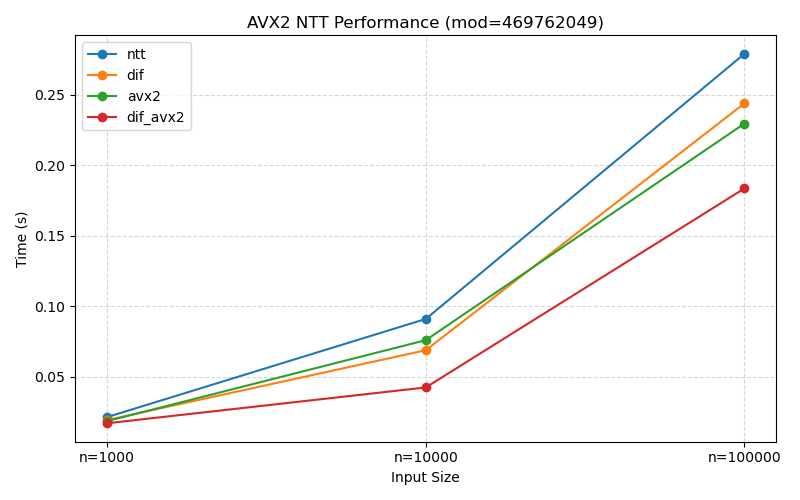
\includegraphics[width=\textwidth]{avx2_469762049.png}
    \caption{AVX2性能对比 (mod=469762049)}
    \label{fig:avx2_469762049}
  \end{subfigure}
  \hfill
  \begin{subfigure}[b]{0.32\textwidth}
    \centering
    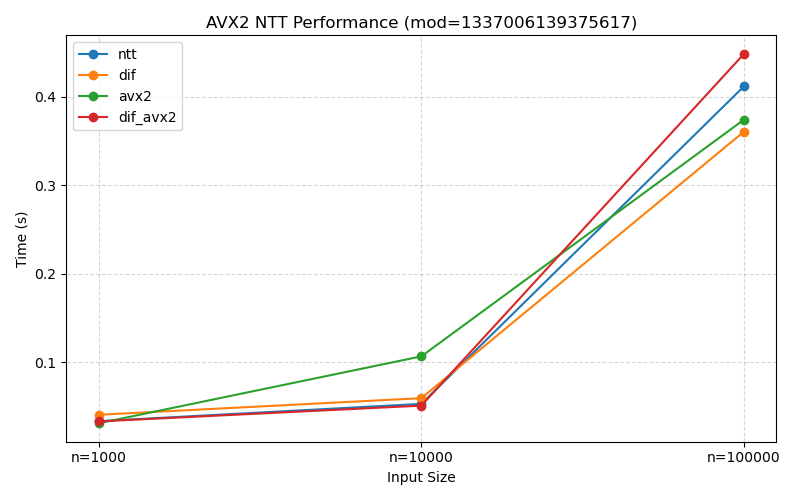
\includegraphics[width=\textwidth]{avx2_1337006139375617.png}
    \caption{AVX2性能对比 (mod=1337006139375617)}
    \label{fig:avx2_1337006139375617}
  \end{subfigure}
  \hfill
  \begin{subfigure}[b]{0.32\textwidth}
    \centering
    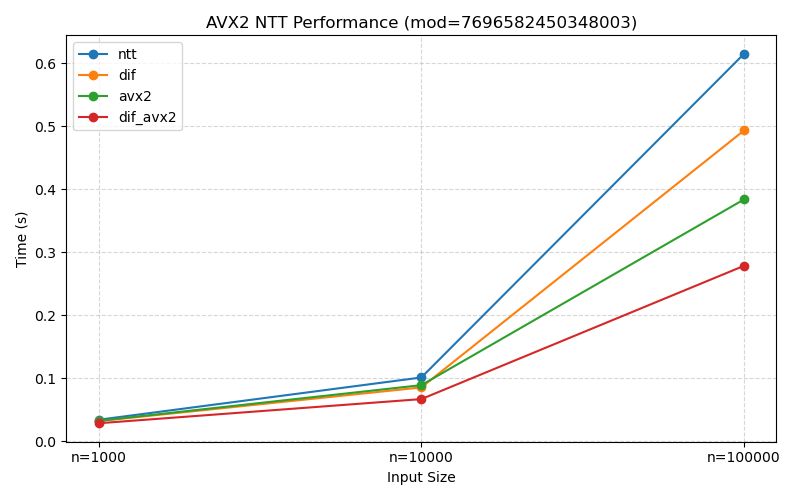
\includegraphics[width=\textwidth]{avx2_7696582450348003.png}
    \caption{AVX2性能对比 (mod=7696582450348003)}
    \label{fig:avx2_7696582450348003}
  \end{subfigure}
  \caption{AVX2平台不同模数下的性能对比}
  \label{fig:avx2_performance}
\end{figure}

\begin{figure}[H]
  \centering
  \begin{subfigure}[b]{0.32\textwidth}
    \centering
    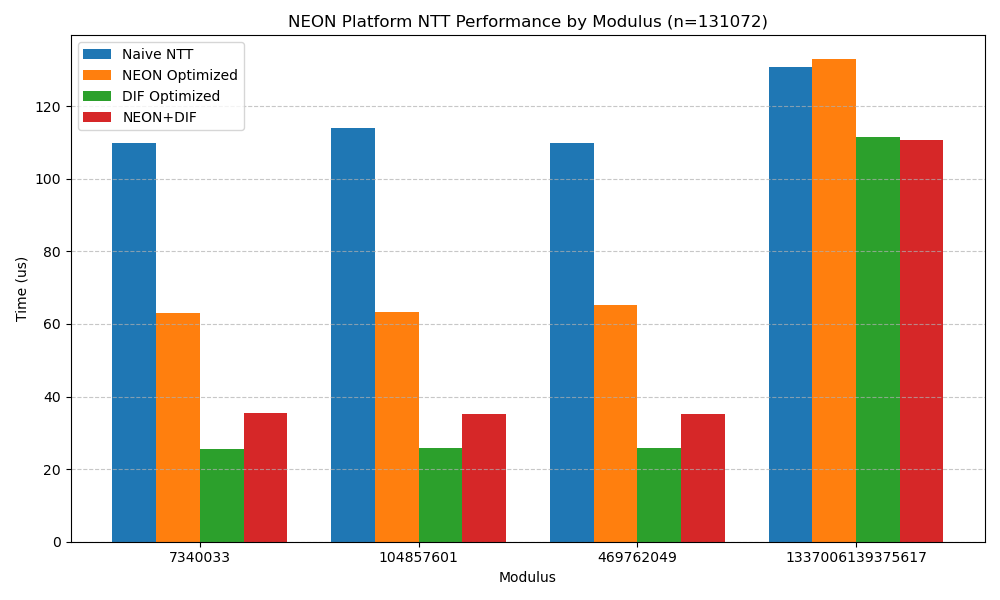
\includegraphics[width=\textwidth]{neon_modulus_comparison.png}
    \caption{NEON平台不同模数对比}
    \label{fig:neon_modulus}
  \end{subfigure}
  \hfill
  \begin{subfigure}[b]{0.32\textwidth}
    \centering
    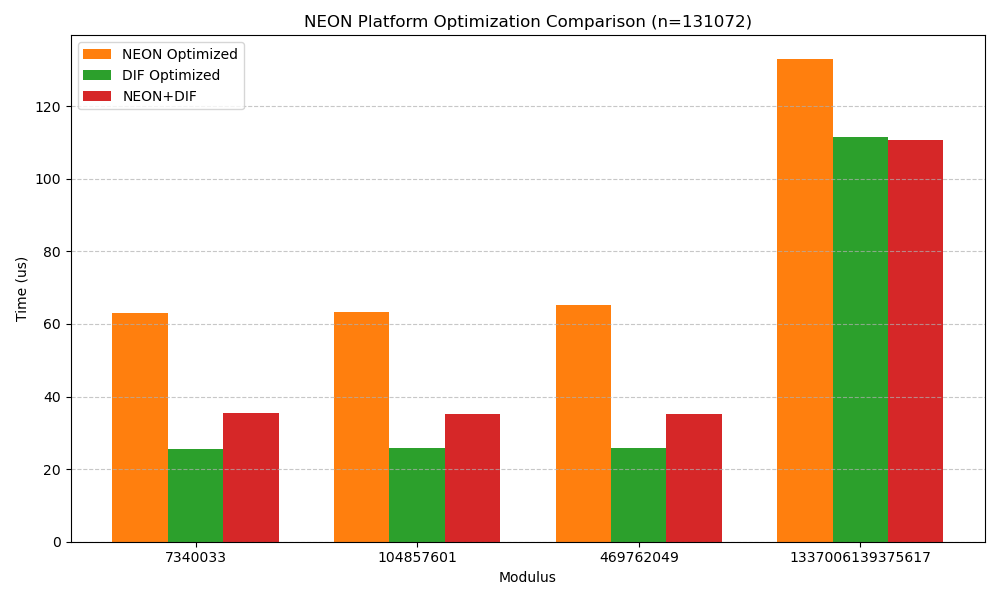
\includegraphics[width=\textwidth]{neon_optimization_comparison.png}
    \caption{NEON平台优化方法对比}
    \label{fig:neon_optimization}
  \end{subfigure}
  \hfill
  \begin{subfigure}[b]{0.32\textwidth}
    \centering
    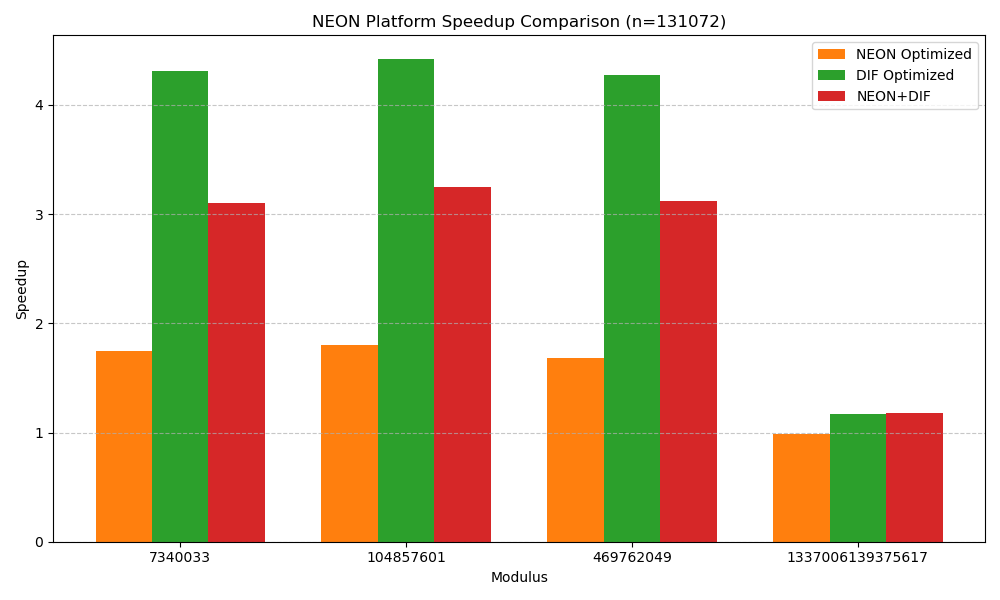
\includegraphics[width=\textwidth]{neon_speedup_comparison.png}
    \caption{NEON平台加速比对比}
    \label{fig:neon_speedup}
  \end{subfigure}
  \caption{NEON平台性能分析图表}
  \label{fig:neon_performance}
\end{figure}

\subsection{简要结果分析}

从图表可以直观看出,不同优化策略在不同平台和模数下表现出显著的性能差异和复杂的交互效应。在AVX2平台(256位宽向量寄存器)上,对于标准模数469762049,DIF+AVX2联合优化(0.183秒)相比朴素实现(0.279秒)能提供约35\%的加速,优于单独使用DIF或AVX2优化。而在NEON平台(128位宽向量寄存器)上,DIF结构优化相较于朴素实现提供了约4倍的加速(从约110微秒降至约25微秒),远超NEON向量化优化的40-45\%提升(从约110微秒降至约63微秒);然而令人意外的是,DIF+NEON联合优化(约35微秒)反而比单独DIF优化(约25微秒)慢约40\%,表明简单叠加优化策略可能导致负面效果。对于超大模数处理,结果展示了两种不同策略的效果:对于不可分解为NTT友好小模数的1337006139375617,SIMD优化实际退化为朴素算法,各实现间观察到的性能差异主要源于系统随机波动,不具算法意义;而对于可分解的7696582450348003,CRT拼接技术成功实现了有效的SIMD优化。这些发现强调了针对不同硬件架构和模数特性,需要采用差异化的优化策略。

\subsection{详细结果分析}

\subsubsection{朴素NTT与优化版本的对比}
\begin{itemize}
  \item 在AVX2平台上,朴素NTT在n=100000时运行时间约为0.28秒,而DIF+AVX2优化减少到约0.18秒,提升性能约35\%。
  \item 在NEON平台上,朴素NTT在大规模数据下(n=131072)运行时间约为110-130微秒,而最佳的DIF优化版本达到了约25微秒,提升了约4倍。
\end{itemize}

\subsubsection{DIF结构优化效果}
\begin{itemize}
  \item 在AVX2平台上,DIF优化在中等规模数据(n=10000)下效果显著,但在大规模数据(n=100000)下略逊于朴素实现,可能受到缓存效应和内存布局的影响。
  \item DIF优化在NEON平台表现最为突出,相比朴素实现提升了4倍多。DIF结构通过改变蝴蝶操作的排列,减少了位翻转和数据重排操作,极大提高了数据局部性和缓存命中率。
\end{itemize}

\subsubsection{SIMD(AVX2/NEON)优化效果}
\begin{itemize}
  \item AVX2优化在不同数据规模下表现不稳定,部分情况下甚至性能下降,这表明向量化优化需要更精细的实现和调整。
  \item NEON优化相比朴素实现有约40-45\%的性能提升,但效果不如DIF结构优化显著。
  \item 对于超出32位范围的大模数1337006139375617,由于不能分解为NTT友好的小模数,所有标记为SIMD优化的实现实际上都退化为朴素NTT算法,因此各实现之间的性能差异主要来自系统负载、内存访问模式、缓存状态等随机因素,不具有算法意义,不应作为优化效果的评判依据。
\end{itemize}

\subsubsection{DIF+SIMD联合优化的效果及异常现象}
\begin{itemize}
  \item 在AVX2平台上,DIF+AVX2联合优化在标准模数下(469762049)能取得最佳效果,表明AVX2的更宽向量(256位)和更丰富的指令集能更好地发挥SIMD的并行优势。
  \item 相比之下,值得注意的是,在NEON平台下,DIF+NEON联合优化(约35微秒)反而比单独DIF优化(约25微秒)慢约40\%。这一反直觉的结果表明,简单叠加两种优化技术并不总是能获得更好的性能。
  \item 分析原因可能包括:
  \begin{enumerate}
    \item NEON指令在DIF结构下可能引入额外的数据依赖和流水线停顿
    \item 向量化操作的额外装载/卸载指令开销可能抵消部分并行收益
    \item 在已经高度优化的DIF结构下,内存访问可能成为主要瓶颈而非计算本身
    \item NEON寄存器数量和宽度限制可能在处理复杂的蝴蝶操作时产生寄存器压力
  \end{enumerate}
\end{itemize}

\subsubsection{模数大小对优化效果的影响}
\begin{itemize}
  \item 对于超大模数1337006139375617,由于超出32位整数范围且不能分解为NTT友好的小模数,所有标记为SIMD优化的实现实际上都使用朴素NTT算法。各实现之间观察到的性能差异主要来自系统负载、内存访问模式、缓存状态等随机因素,不具有算法意义,不应作为优化效果的评判依据。
  \item 对于7696582450348003模数,通过将其分解为两个NTT友好的小模数7340033和104857601,然后分别进行SIMD加速计算,再通过中国剩余定理合并结果,成功实现了SIMD优化,展示了算法创新在处理特殊模数时的重要性。
  \item 这种对比突显了针对不同模数特性采用差异化优化策略的必要性:对于标准模数可直接应用SIMD优化,对于可分解为NTT友好小模数的大模数可采用CRT拼接技术,而对于不可分解的超大模数则需要开发专门的大整数算法。
\end{itemize}

\subsubsection{平台特性与优化策略的关系}
\begin{itemize}
  \item AVX2平台(256位向量宽度)下,结合结构优化和SIMD并行能获得最佳效果。
  \item NEON平台(128位向量宽度)下,数据局部性优化(如DIF)比SIMD并行更重要。
  \item 这表明优化策略应根据目标平台特性和问题规模灵活调整,而非简单套用。
\end{itemize}

\section{总结与展望}

\subsection{主要发现}
本实验通过在x86和ARM两种平台上实现并测试NTT的多种优化策略,得到了以下主要发现:

\begin{enumerate}
  \item NTT优化将多项式乘法复杂度从$O(n^2)$降低到$O(n\log n)$,在大规模数据下提供了显著加速。
  \item 不同平台上最有效的优化策略存在差异:AVX2平台下DIF+SIMD联合优化在标准模数下表现最佳,而NEON平台下DIF结构优化最有效。
  \item 硬件特性(如向量宽度、缓存大小)与算法结构的匹配度对性能影响显著。
  \item 超大模数处理需要分类处理:对于可分解为NTT友好小模数的大模数(如7696582450348003)可采用CRT拼接技术实现SIMD优化,而对于不可分解的超大模数(如1337006139375617)则需要退回到朴素NTT算法,此时观察到的性能差异主要来自系统随机波动,不具有算法意义。
  \item 优化技术的简单叠加可能产生负面效果,需要针对具体平台和问题特性进行精细调整。
\end{enumerate}

\subsection{未来工作}
基于本实验的发现,未来可进一步探索以下方向:

\begin{enumerate}
  \item \textbf{算法结构优化}:探索更适合SIMD向量化的NTT变体,如四分法或更高基数的蝴蝶变换。
  \item \textbf{高效模乘算法}:深入研究Barrett/Montgomery等规约方法在SIMD环境下的优化实现。
  \item \textbf{多层次并行}:结合SIMD、多线程、MPI等多种并行技术,实现更高效的NTT实现。
  \item \textbf{专用硬件加速}:探索GPU、FPGA等专用硬件对NTT的加速潜力。
  \item \textbf{大模数优化}:开发更高效的大整数模乘算法以应对同态加密中常见的超大模数场景。
\end{enumerate}

本实验为多项式乘法的高效实现提供了重要的经验和指导,对于理解现代处理器架构下的算法优化具有重要参考价值。在未来的密码学和同态加密应用中,基于本实验的优化策略可以大幅提升系统性能,为隐私保护计算提供更强大的技术支持。

\clearpage
\phantomsection
\addcontentsline{toc}{section}{参考文献}
% 使用natbib配合biblatex的方式处理参考文献
\renewcommand{\bibname}{参考文献}
\nocite{*} % 显示全部参考文献,即使未被引用
\bibliography{reference}

\clearpage
\phantomsection
\appendix
\addcontentsline{toc}{section}{附录A}
\section*{附录A:NEON平台实验结果截图}
\renewcommand{\thesubsection}{A.\arabic{subsection}}

% 重置图表计数器并修改图表编号格式
\setcounter{figure}{0}
\renewcommand{\thefigure}{A.\arabic{figure}}

\subsection{朴素NTT实现}
\begin{figure}[H]
  \centering
  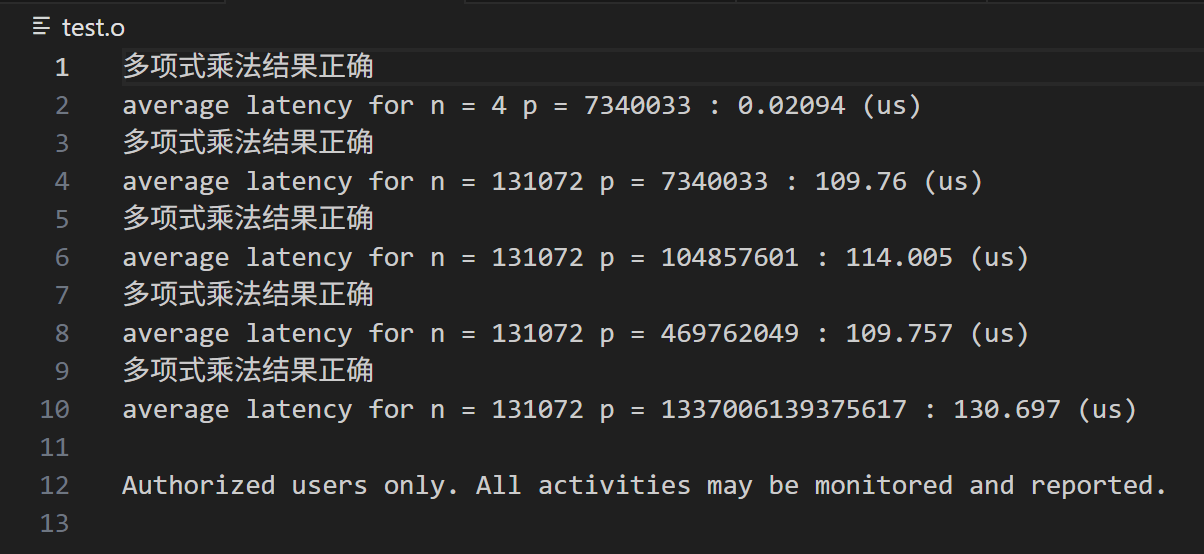
\includegraphics[width=0.7\textwidth]{ntt.png}
  \caption{朴素NTT实现性能}
  \label{fig:ntt_screenshot}
\end{figure}

\subsection{DIF优化实现}
\begin{figure}[H]
  \centering
  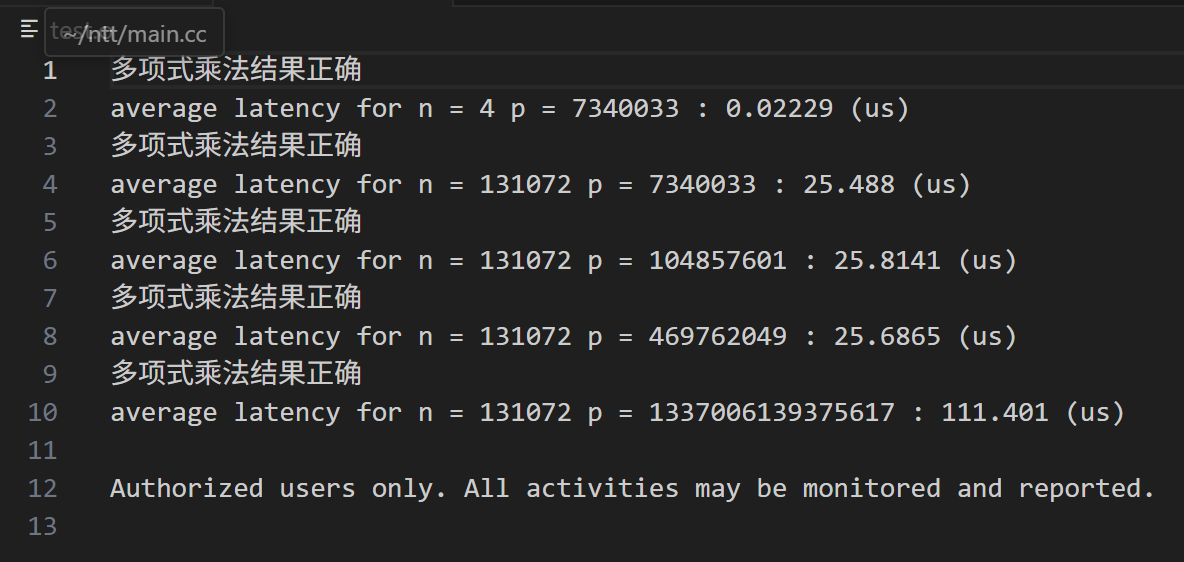
\includegraphics[width=0.7\textwidth]{dif.png}
  \caption{DIF优化实现性能}
  \label{fig:dif_screenshot}
\end{figure}

\subsection{NEON优化实现}
\begin{figure}[H]
  \centering
  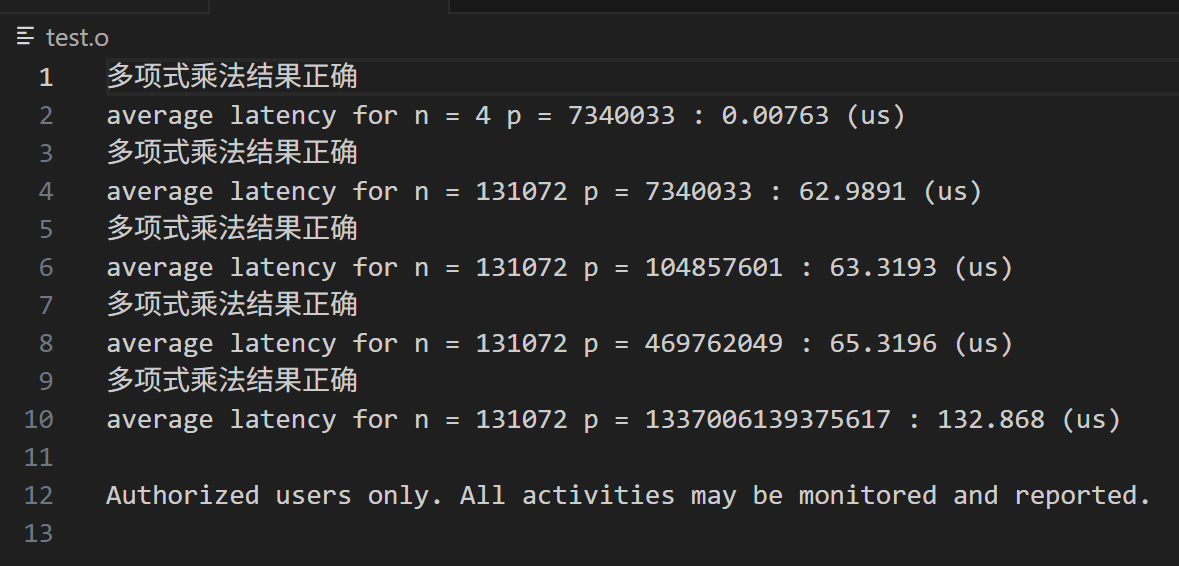
\includegraphics[width=0.7\textwidth]{neon.png}
  \caption{NEON优化实现性能}
  \label{fig:neon_screenshot}
\end{figure}

\subsection{DIF+NEON联合优化}
\begin{figure}[H]
  \centering
  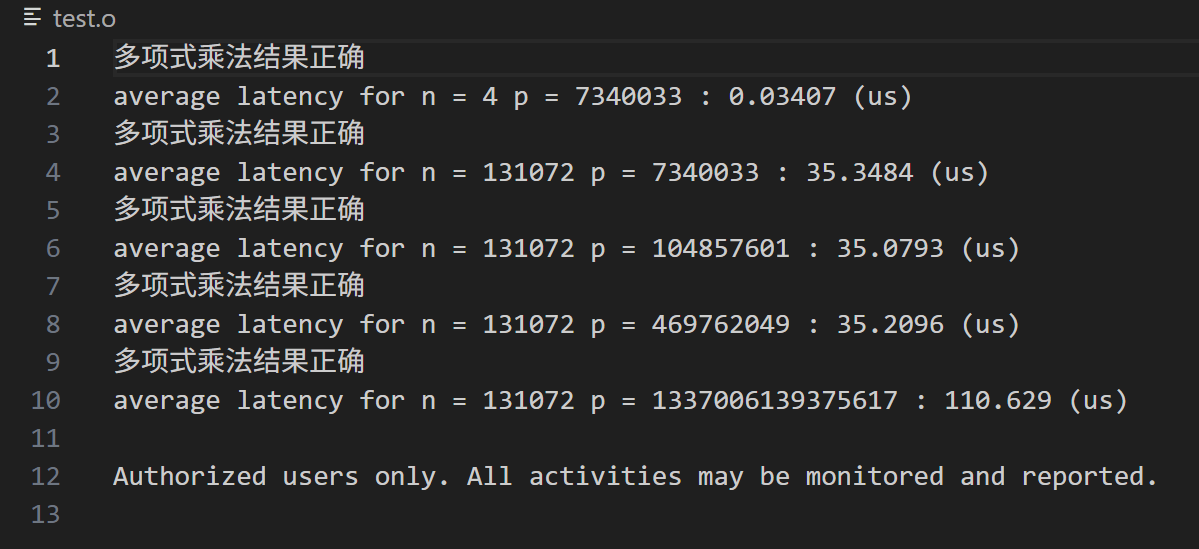
\includegraphics[width=0.7\textwidth]{dif_neon_full.png}
  \caption{DIF+NEON联合优化性能}
  \label{fig:dif_neon_full_screenshot}
\end{figure}

\end{document} 